\documentclass{article}
\usepackage[T1]{fontenc}

\title{Parametric bootstrap for linear and generalized linear models}
\author{Ulrich Halekoh and S�ren H�jsgaard}

\usepackage{Sweave}
\begin{document}
\renewenvironment{Schunk}{\linespread{.85}\small}{}
 
\setkeys{Gin}{width=0.5\textwidth} %s�t figurst�rrelse i Sweave

\maketitle
%\fxnote{where should this line be placesd?}

\section{budworm}
\label{sec:logist-regr-budw}

\subsection{Linear regression}
\label{sec:linear-regression}


\begin{Schunk}
\begin{Sinput}
> data(budworm, package='LiSciData')
> library(lattice)
> par(mfrow=c(1,2))
> print(xyplot(ndead/20~log(dose), groups=sex, data=budworm,
+              type="b", auto.key=T))
> 
\end{Sinput}
\end{Schunk}
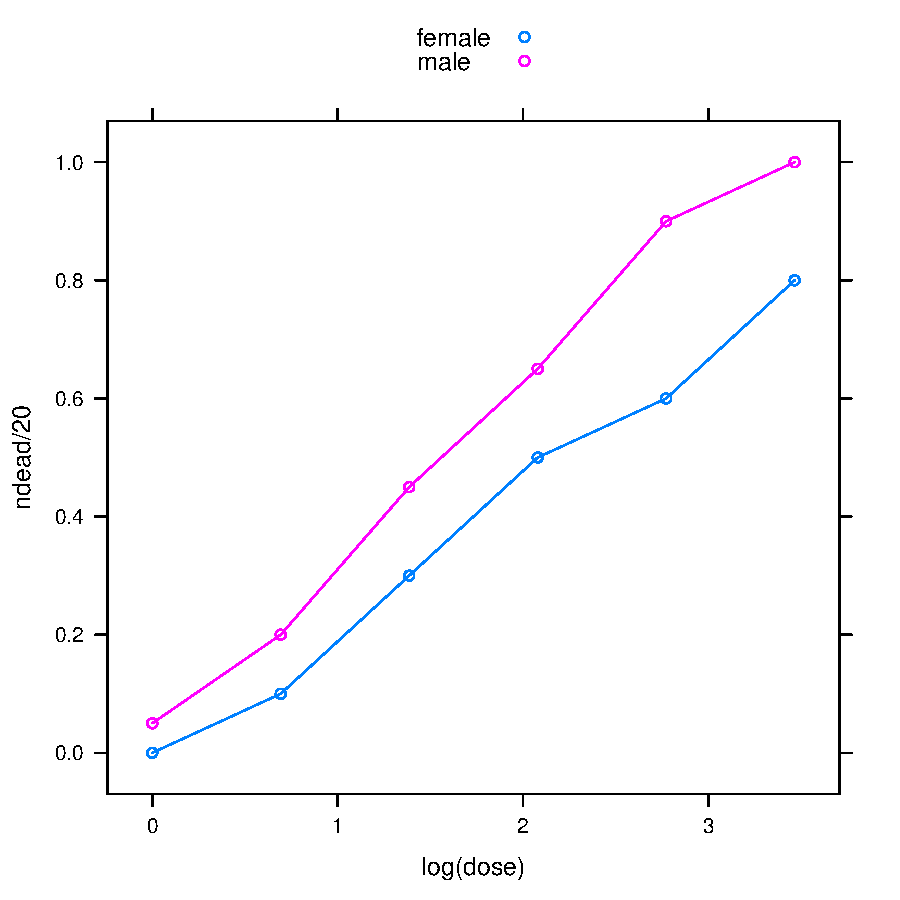
\includegraphics{fig/mm-002}




\begin{Schunk}
\begin{Sinput}
> lm1 <- lm(ndead/20~sex+log(dose), data=budworm) 
> lm0 <- update(lm1,.~.-sex)
> PBmodcomp(lm1, lm0, nsim=999)
\end{Sinput}
\begin{Soutput}
Parametric bootstrap test; bootstrap samples: 999 computing time: 3.09 sec.
large : ndead/20 ~ sex + log(dose)
small : ndead/20 ~ log(dose)
             stat df   p.value   ddf
LRT      16.93364  1 0.0000387    NA
PBtest   16.93364 NA 0.0010010    NA
PBkd     16.93364 NA 0.0010021    NA
Gamma    16.93364 NA 0.0007067    NA
Bartlett 12.30399  1 0.0004520    NA
F        16.93364  1 0.0040813 7.315
\end{Soutput}
\begin{Sinput}
> anova(lm1,lm0)
\end{Sinput}
\begin{Soutput}
Analysis of Variance Table

Model 1: ndead/20 ~ sex + log(dose)
Model 2: ndead/20 ~ log(dose)
  Res.Df      RSS Df Sum of Sq      F    Pr(>F)    
1      9 0.024256                                  
2     10 0.099464 -1 -0.075208 27.905 0.0005054 ***
---
Signif. codes:  0 '***' 0.001 '**' 0.01 '*' 0.05 '.' 0.1 ' ' 1 
\end{Soutput}
\end{Schunk}


\subsection{Logistic regression}
\label{sec:logistic-regression}

\begin{Schunk}
\begin{Sinput}
> library(lattice)
> print(xyplot(log((ndead+.5)/(20-ndead+.5))~log(dose), groups=sex, data=budworm,
+              type="b", auto.key=T))
\end{Sinput}
\end{Schunk}
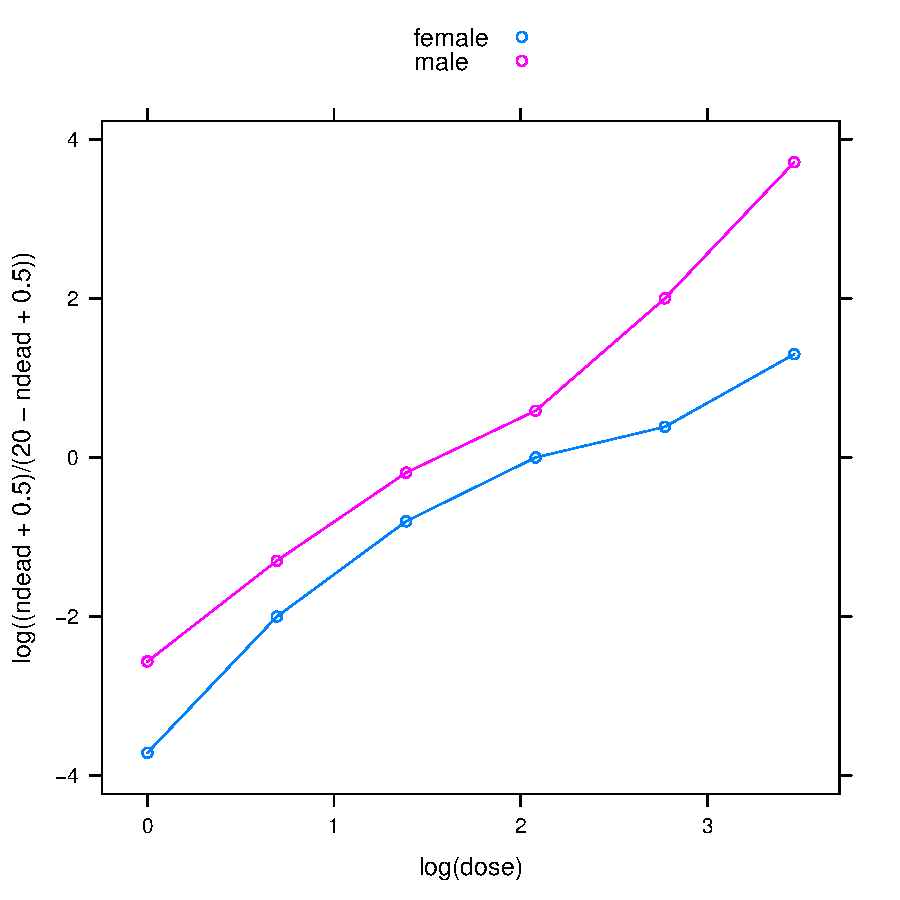
\includegraphics{fig/mm-004}


\begin{Schunk}
\begin{Sinput}
> budworm <- transform(budworm, logdose=log(dose))
> lreg1 <- glm(cbind(ndead,ntotal-ndead)~sex+logdose,
+         data=budworm, family=binomial(link=logit))
> lreg0 <- update(lreg1,.~.-sex)
> PBmodcomp(lreg1, lreg0, nsim=999)
\end{Sinput}
\begin{Soutput}
Parametric bootstrap test; bootstrap samples: 947 computing time: 4.51 sec.
large : cbind(ndead, ntotal - ndead) ~ sex + logdose
small : cbind(ndead, ntotal - ndead) ~ logdose
              stat df   p.value    ddf
LRT      10.226968  1 0.0013840     NA
PBtest   10.226968 NA 0.0021119     NA
PBkd     10.226968 NA 0.0021110     NA
Gamma    10.226968 NA 0.0014865     NA
Bartlett  9.531979  1 0.0020192     NA
F        10.226968  1 0.0033005 29.431
\end{Soutput}
\end{Schunk}



\end{document}




